\documentclass{scrartcl}

\usepackage{microtype}
\usepackage{hyperref}
\usepackage[british]{babel}
\usepackage{tabularx}
\usepackage{booktabs}
\usepackage{siunitx}
\usepackage{graphicx}
\usepackage{datetime}
\usepackage[backend=biber,style=ieee]{biblatex}
\usepackage{filecontents}
\usepackage{subcaption}
\usepackage{float}

\setcounter{tocdepth}{\subsectiontocdepth}

\hypersetup{pdftitle={A gamified approach to workplace diversity and inclusion — Project definition document},
  pdfauthor={Mohammad Abbas, Olamide Olufayo, Noah Tarr, Yash Vedak, Bhavdeep Virk and Awaale Yussuf},
  pdfsubject={Inclusive workplaces and training},
  hidelinks}

\newcommand{\email}[1]{\texttt{\href{mailto:#1}{#1}}}
\DeclareSIUnit[quantity-product = ]\percent{\char`\%}

\titlehead{COM2027 project definition document}
\subject{Inclusive workplaces and training}
\title{A gamified approach to workplace diversity and inclusion}
\author{
  Mohammad Abbas\\\email{m-00104@surrey.ac.uk}
  \and
  Olamide Olufayo\\\email{oo01267@surrey.ac.uk}
  \and
  Noah Tarr\\\email{nt00654@surrey.ac.uk}
  \and
  Yash Vedak\\\email{yv00051@surrey.ac.uk}
  \and
  Bhavdeep Virk\\\email{bv00152@surrey.ac.uk}
  \and
  Awaale Yussuf\\\email{ay00487@surrey.ac.uk}
}
\publishers{Dr Jon Machtynger\\\email{j.machtynger@surrey.ac.uk}}

\newcommand{\mkbibnodate}{n\adddot d\adddot}
\AtEveryCitekey{\iffieldundef{labelyear}{\restorefield{labelyear}{\mkbibnodate}}{}}
\AtEveryBibitem{\iffieldundef{labelyear}{\restorefield{year}{\mkbibnodate}}{}}

\begin{filecontents*}[overwrite]{refs.bib}
@online{openai-api,
    author = {OpenAI},
    url = {https://openai.com/api},
    urldate = {2025-03-18}
}

@online{perspective-api,
author = {{Google LLC}},
shortauthor = {Google},
url = {https://perspectiveapi.com},
urldate = {2025-03-18}
}

@software{django,
title={Django},
author={Adrian Holovaty and Simon Willison and others},
organization={{Django Software Foundation}},
url={https://djangoproject.com},
urldate = {2025-03-18}
}

@software{sqlite,
title={SQLite},
author={D.\ Richard Hipp and others},
url={https://sqlite.org},
urldate = {2025-03-18},
version={3}
}

@software{javascript,
title={JavaScript},
organization={Oracle Corporation}
}

@software{react,
title={React},
author={{Meta Platforms} and others},
url={https://react.dev},
urldate = {2025-03-18}
}

@software{supermemo,
title={SuperMemo},
author={Piotr Wozniak and others},
url={https://super-memory.com},
urldate = {2025-03-18}
}

@software{anki,
title={Anki},
author={Damien Elmes and others},
url={https://apps.ankiweb.net},
urldate = {2025-03-18}
}

@online{whatsapp,
title={WhatsApp Messenger},
author={{Meta Platforms}},
date={2025},
url={https://whatsapp.com},
urldate = {2025-03-18}
}

@online{teams,
title={Microsoft Teams},
author={{Microsoft}},
url={https://teams.microsoft.com},
urldate={2025-03-18}
}

@software{docker,
title={Docker},
author={Solomon Hykes and others},
organization={Docker, Inc.},
url={https://docker.com},
urldate={2025-03-18}
}

@online{discord,
title={Discord},
author={Discord},
url={https://discord.com},
urldate={2025-03-18}
}

@online{gitlab,
title={GitLab},
author={GitLab},
url={https://about.gitlab.com},
urldate={2025-03-18}
}

\end{filecontents*}

\addbibresource{refs.bib}

\begin{document}
\maketitle
\newpage
\tableofcontents
\section{Project charter}
\subsection{Business need and environment}
Workplace diversity, equity and inclusion (DEI) training often fails to meaningfully engage employees, resulting in minimal improvements to workplace inclusivity.
Conventional DEI methods are often viewed as time-consuming, overly general and difficult to measure in terms of impact.
Organisations need a solution to make DEI training more engaging and interactive and to measure the impact it has on its employees.

\subsection{Project objective}
The purpose of this project is to develop a gamified DEI learning platform that uses interactive and captivating techniques to improve DEI training. The platform will make use of AI-driven adaptive learning, spaced repetition and quizzes to boost employee engagement, personalise the learning experience and improve knowledge retention.

\subsection{Constraints}
Three preliminary limitations have been assigned, and our application will adhere to them:
\begin{enumerate}
\item To run inside a Docker \parencite{docker} container with all necessary libraries included.
\item To make use of at least two external APIs (in our case: the OpenAI API \parencite{openai-api} and the Perspective API \parencite{perspective-api})
\item To deploy a real-time client-server streaming component that goes beyond request-response by sending emails to remind the user to log in to the app.
\end{enumerate}

The short-term scope of the project will be to make a platform with the following core functionalities.

\begin{enumerate}
\item AI-powered adaptive learning for personalised training.
\item Gamification elements, such as quizzes and a leaderboard.
\item A spaced repetition system for reinforcing DEI concepts.
\end{enumerate}

However, there are some items that are outside the current short-term scope of the project:
\begin{enumerate}
\item Full scale deployment across multiple organisations and industries.
\item Personalised customisation for different industries.
\end{enumerate}

\subsubsection{Resources}
\begin{enumerate}
\item The team: Mohammad Abbas, Yash Vedak, Awaale Yussuf, Noah Tarr, Bhavdeep Virk and Olamide Olufayo.
\item A server that can handle server-side processing.
\end{enumerate}

\subsection{Dependencies}
The project will depend on the functionality of external APIs:
\begin{enumerate}
\item The OpenAI API \parencite{openai-api} will be used to generate questions and their answers.
\item The Perspective API \parencite{perspective-api} will be used to filter questions for potentially biased language.
\end{enumerate}

\subsection{Project stakeholders}
The users of our software are stakeholders.
They will want the software to be engaging, informational and easy to use.

\par
Minority groups are stakeholders.
They will want the software to be effective at getting across accurate knowledge.

\par
Dr Jon Machtynger is our project's sponsor.
He will oversee our project and provide us with guidance and support to ensure the successful development of this project.

\section{Project description}
\subsection{Introduction}
This project focuses on promoting inclusivivity in workplaces and training within the workforce, where diversity training remains a challenge in many workplaces, being unengaging and involving passive engagement.

\par
We aim to address this by offering an interactive platform where employees can participate in courses covering topics such as culture, socioeconomic background, gender, race, sexuality and disabilities.

\subsection{Features}
\subsubsection{Streak system}

The streak system will encourage users to log in consistently, by tracking the number of consecutive days during which they access the platform.

\par
Users will receive incentives such as badges, to further gamify the learning experience.
Additionally, notifications will be sent to remind users to keep their streaks going, reinforcing engagement over time.

\subsubsection{Email reminder system}
To further support user retention, the email reminder system will send automated emails to individuals who haven't logged in for a set period.
These reminders will be customisable in frequency, encouraging users to return and to continue consistently learn about DEI.

\subsubsection{Profile system}
The profile system will allow users to view key details about their colleagues within the organisation. This could include facts about colleagues, like their beliefs and orientations. This would be something that users can manage and hide if they wanted.

\subsubsection{Daily fact system}

A daily fact system will provide users with a new DEI-related fact each day upon logging in. These facts can be curated from reliable sources and would provide further incentive for daily log ins.

\subsubsection{Courses}

For structured learning, the platform will feature sourses, where users can select DEI-related topics to study. Course questions will be mainly written by humans; however, some aspects will be dynamically generated using the OpenAI API \parencite{openai-api} and then filtered through the Perspective API \parencite{perspective-api} to ensure clarity, and filter potentially biased language from the questions. Organisations can assign specific courses to users as required learning, ensuring that employees or members complete essential training. Additionally, users will have the freedom to explore optional courses based on their interests, allowing for personalised learning paths.

\subsubsection{Spaced repetition system}

To enhance long-term retention, the platform will incorporate a spaced repetition system.
This system will intelligently reintroduce key DEI concepts at optimal intervals.
By adjusting the review frequency according to individual progress, the system ensures that users retain important information over time, reinforcing knowledge in a natural and effective manner.

\par
The system will include a daily check-up feature that uses spaced repetition to ask relevant questions from a user’s active courses.
This ensures continuous engagement and reinforcement of key concepts, making learning an ongoing process rather than a one-time event.

\subsubsection{Leaderboard system}

The platform will include a leaderboard system to encourage engagement and friendly competition among users.
There will be two separate leaderboards:

\begin{description}
\item[Points Leaderboard] Tracks points earned through course completions, quiz performance, and overall engagement with the platform. This incentivises active participation and consistent learning.
\item[Streak Leaderboard] Tracks the longest active streaks of users, highlighting those who have maintained consistent daily logins. This encourages long-term commitment to the platform
\end{description}

\subsubsection{Newsfeed system}

The platform will feature a newsfeed system that highlights special days, observances, and key events related to DEI. This feed will showcase important cultural, historical and awareness days, such as International Women’s Day, Pride Month or World Mental Health Day. Users can engage with these posts by learning more about the significance of each event.

\subsection{Account management}
Employees will automatically have their accounts, meaning they can use the application and participate in the courses and other features.
With these accounts employees can create their passwords, making sure they follow password standards.
The account will contain a range of information about the employees, such as their name, age, ethnicity or background.

\par
This confidential information will be protected through Django \parencite{django} (see section~\ref{sec:tech}), using its authentication systems.
We will measure how easy it is to edit employees' accounts and that access to their data is restricted to the appropriate users.

\par
We will test this by running unit tests to check account security and that accounts display the correct information and carrying out in-person user testing, trying to get employees to have a smooth experience with their accounts.

\section{Technical approach}
We will use the JavaScript language \parencite{javascript} and the React framework \parencite{react} for the frontend, and the Python programming language and the Django\label{sec:tech} web framework \parencite{django} (with its built-in SQLite \parencite{sqlite} database) for the backend.

\par
The user's command of each topic will be tracked using a speced repetition system \parentext{similar to those of SuperMemo \parencite{supermemo} or Anki \parencite{anki}} and tested by multiple-choice questions generated by a GPT model, using the OpenAI API \parencite{openai-api}.

\par
We will host our code on GitLab \parencite{gitlab}.

\section{Team charter and rules of engagement}
\subsection{Engagement}
Effective communication is key to ensuring the success of our project.
To ensure communication and collaboration within the group and to make sure that important information is acknowledged by everyone, the following rules of engagement will be followed:

\begin{description}
\item[Acknowledging messages]Team members are required to leave a thumbs-up reaction on all important messages and announcements to confirm they have read them. This applies specifically to messages where they have been tagged (``@'') individually or when an ``@everyone'' announcement is made.
\item[Responsiveness]When a team member is reached out to directly, they are expected to respond within  24 hours  unless they have communicated prior commitments that may delay their response time.
\end{description}

\subsection{Weekly meetings}
To maintain regular communication and project progress, we will have a weekly in-person meeting every Monday at \formattime{16}{0}{0}.
\par
Attendance is expected from all team members unless prior notice is given.

\par
Any other meetings outside of the scheduled Monday session will be held on Discord \parencite{discord} as needed.

\par
Meeting minutes will be recorded and shared with those unable to attend.


\subsubsection{Meeting expectations}
All team members should arrive on time and be prepared with updates on their assigned tasks.
If a team member is unable to attend due to a valid reason, they must inform the team in advance.

\subsection{Communication}
We will use WhatsApp \parencite{whatsapp} as the primary communication medium for quick discussions, updates and urgent messages.
Discord \parencite{discord} will be used only for facilitating online meetings.
If any team member prefers a different platform for individual outreach, they must communicate their preference in advance so that the team can accommodate their needs.

\subsection{Scaling form and team evaluation criteria}
To ensure fairness and accountability within the team, we will assess contributions based on a scaling form.
Our project sponsor has granted us the flexibility to determine our own evaluation criteria.

\par
The following key factors have been agreed upon.

\begin{description}
\item[Response time] Team members must respond to messages within 24 hours, unless they have previously-stated commitments that would delay responses.
\item[Quality of work] Deliverables should be completed to a high standard, requiring minimal revisions and ensuring that the work is immediately usable by the team.
\item[Timely completion of work] Tasks must be completed by the agreed deadlines as set in our meetings. Delays should be communicated in advance so that contingency plans can be made.
\item[Meeting attendance] Attendance at weekly meetings is required unless prior commitments have been communicated. Missing meetings without notice will be considered a failure to engage with the team.
\end{description}

\subsection{Conflict resolution and accountability}
To maintain a positive and productive team dynamic, all members are expected to address concerns respectfully and constructively.

\par
If issues should arrive, the team will first attempt resolution through open discussion.
If necessary, the project manager will mediate.
Persistent issues affecting the project's progress will be escalated to the project sponsor.

\par
By adhering to these rules, we aim to ensure that our team operates efficiently, meets deadlines and has a collaborative working environment.
If any team member has suggestions for improvements to these engagement rules, they are encouraged to bring them up in our meetings.

\iffalse
\section{Project management and methodology}

\clearpage
\section{Work plan}
\iffalse To ensure the smooth execution of our project, our team will hold at least one weekly meeting to review our progress, assess whether we have met our milestones, and address any roadblocks or necessary adjustments. If an in-person meeting isn't possible for a team member, they can still participate via Microsoft Teams \parencite{teams}, ensuring they stay informed and engaged. In addition to our weekly meetings, we will incorporate group or paired programming sessions, allowing team members to gain insight into each other's work and collaborate effectively. This approach will help us work in parallel, streamline development and maintain steady progress throughout the project.\fi

\par
See figure~\ref{fig:work-plan}.
\begin{figure}[h]
  \centering
  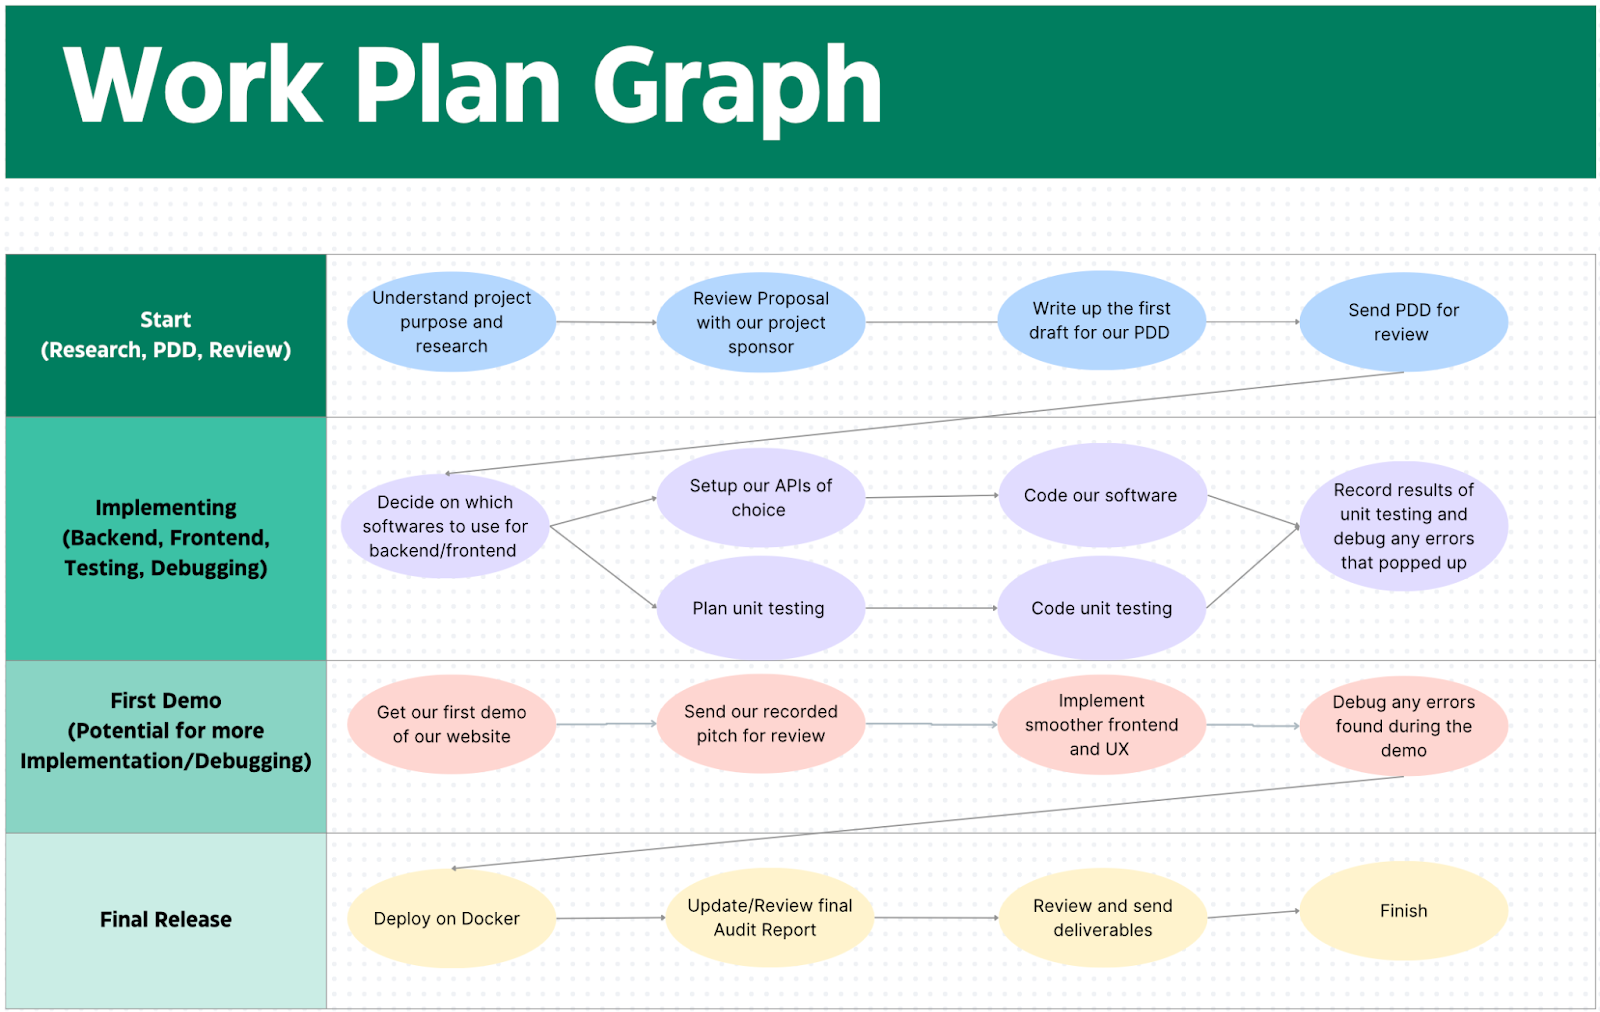
\includegraphics[width=0.7\textwidth]{work-plan.png}
  \caption{Our plan represented as a directed acyclic graph, with labelled subgraphs}
  \label{fig:work-plan}
\end{figure}
\fi

\section{Team roles}
As the \textbf{team lead}, Yash
\begin{itemize}
\item oversees the project,
\item ensures that deadlines are met,
\item facilitates communication, both within the group and with the sponsor,
\item keeps the documentation up to date and
\item performs miscellaneous work when required.
\end{itemize}

As the \textbf{technical lead} and \textbf{deputy team lead}, Noah
\begin{itemize}
\item provides technical assistance across all aspects of the project,
\item manages Docker \parencite{docker},
\item collates, edits and typesets all formal communication with the client and
\item assumes the team lead's responsibilities in his absence.
\end{itemize}

As the \textbf{frontend developer}, Bhavdeep
\begin{itemize}
\item is responsible for the design and implementation of the user interface.
\end{itemize}

As the \textbf{backend developer}, Ola
\begin{itemize}
\item develops and maintains the backend, excepting the functionality for which Awaale or Abbas is reponsible.
\end{itemize}

As the \textbf{AI and content developer}, Awaale
\begin{itemize}
\item develops and refines the system of AI-generated questions and
\item ensures that the AI-generated content aligns with the project's goals.
\end{itemize}

As the \textbf{database administrator}, Abbas
\begin{itemize}
\item designs and maintains the database.
\end{itemize}

The aforesaid notwithstanding, each team member is expected to collaborate across different roles as needed and to provide support to ensure that the project progresses smoothly.

\section{Project timeline}
\subsection{Week 1}
\begin{itemize}
\item Finalise project scope and requirements.
\item Assign team roles.
\item Set up communication channels.
\item Conduct initial research on system architecture.
\end{itemize}

\subsection{Weeks 2 and 3}
\begin{itemize}
\item Begin development of the system of AI-generated questions.
\item Start setting up the SQL database.
\item Begin frontend UI design mockups.
\item Set up Django backend skeleton.
\item Implement frontend layout.
\item Configure the Docker \parencite{docker} environment.
\end{itemize}

\subsection{Weeks 4 and 5}
\begin{itemize}
\item Get the backend's database connection working.
\item Continue improving AI-generated questions.
\item Finalise initial frontend mockups.
\item Improve database performance.
\end{itemize}

\subsection{Weeks 6}
\begin{itemize}
\item Prepare for the meeting with our sponsor.
\item \textbf{Submit Project Definition Document (March 18).}
\item Implement the backend API, to serve questions to the frontend.
\item Ensure that the database can handle large-scale queries efficiently.
\end{itemize}

\subsection{Week 7}
\begin{itemize}
\item \textbf{Meet with sponsor (March 27).}
\item Connect the frontend and backend.
\item Implement basic user authentication and session management.
\item Conduct initial testing of the full system's functionality.
\end{itemize}

\subsection{Week 8}
\begin{itemize}
\item Implement answer submission and the scoring system.
\item Improve AI-generated question quality based on feedback from the sponsor.
\item Enhance database efficiency for handling of queries.
\end{itemize}

\subsection{Weeks 9 and 10}
\begin{itemize}
\item Refine the UI.
\item Conduct testing and refinement of the system.
\item Debug.
\end{itemize}

\subsection{Week 11}
\begin{itemize}
\item Implement feedback from the testing phase.
\item Ensure that logs and error handling are in place.
\item Conduct a second round of testing.
\end{itemize}

\subsection{Week 12}
\begin{itemize}
\item Make final bug fixes and performance improvements.
\item Polish the frontend design and user experience.
\item Perform a security review.
\end{itemize}

\subsection{Week 13}
\begin{itemize}
\item Test and deploy.
\item Prepare project submission materials.
\item Ensure that the documentation is finalised and reviewed.
\end{itemize}

\subsection{Week 14}
\begin{itemize}
\item \textbf{Finally submit the project (May 13).}
\end{itemize}

This serves as a guide for the pace of our project --- our actual internal deadlines may differ slightly.

\section{Risk assessment}
See table~\ref{tab:risk}.
\begin{table}
  \centering
  \sisetup{table-format=2.0, table-number-alignment=center, table-auto-round=true}
  \begin{tabularx}{\textwidth}{X S l r X}
    \toprule
    Risk & {Probability} & Severity & Rank & Action \\
    \midrule
    A team member misunderstanding their responsibilities & 25\% & High&1&The project manager will require each team member to affirm that they understand what is required of them when they are so told.\\
    Code loss & 30\% & Medium&2& We will develop on our own computers, frequently uploading to and downloading from GitLab \parencite{gitlab}. Also, each of us will make a manual backup at least once per week.\\
    A team member no longer contributing & 4\% & High &3& We will remain in frequent mutual communication. If a team member has been silent, the project manager (or, in their (very unlikely) case, someone else) will endeavor to determine whether they will continue to contribute.\\
    An API we depend on receiving breaking changes, ceasing operation or increasing significantly more & 2\% & Low&4&We will make some effort to understand what each API we use accomplishes, beyond merely its interface.\\
    \bottomrule
  \end{tabularx}
  \caption{Our risks, somewhat quantitatively analysed}
  \label{tab:risk}
\end{table}
\clearpage
\printbibliography
\appendix
\section{IKEEP badges}
See figure~\ref{fig:badges}.
\begin{figure}
  \centering
  \label{fig:badges}
  \begin{subfigure}[b]{0.3\textwidth}
    \centering
    \href{https://openbadgefactory.com/v1/assertion/20767cc55d7f0a2156b97ac4a8edaa78c8b32ba1}{
\includegraphics[width=\textwidth]{badge.png}}
    \caption{Mohammad Abbas's}
  \end{subfigure}
  \hfill
  \begin{subfigure}[b]{0.3\textwidth}
    \centering
    [Missing]\vspace{5em}
    \caption{Olamide Olufayo's}
  \end{subfigure}
  \hfill
  \begin{subfigure}[b]{0.3\textwidth}
    \centering
    \href{https://openbadgefactory.com/v1/assertion/def847fc189ca5ac8503c9a52d31c6d0d487e688.html}{
\includegraphics[width=\textwidth]{badge.png}}
    \caption{Noah Tarr's}
  \end{subfigure}
  
  \vspace{1em}
  
  \begin{subfigure}[b]{0.3\textwidth}
    \centering
    \href{https://openbadgefactory.com/v1/assertion/ac4ade6eee30da38d08523ef9e581771cd93e426}{
\includegraphics[width=\textwidth]{badge.png}}
    \caption{Yash Vedak's}
  \end{subfigure}
  \hfill
  \begin{subfigure}[b]{0.3\textwidth}
    \centering
    \href{https://openbadgefactory.com/v1/assertion/dfc254a7236439b7b2cacfabf2e64741e3a81b50}{
\includegraphics[width=\textwidth]{badge.png}}
    \caption{Bhavdeep Virk's}
  \end{subfigure}
  \hfill
  \begin{subfigure}[b]{0.3\textwidth}
    \centering
    \href{https://openbadgefactory.com/v1/assertion/5714857e909a59b55354ccc68f78bf2139204d1c}{
\includegraphics[width=\textwidth]{badge.png}}
    \caption{Awaale Yussuf's}
  \end{subfigure}
  \caption{Our IKEEP badges}
  \label{fig:badges}
\end{figure}
\end{document}